% Existing selection figure is included directly, without changing data.
\subsection{Preprocessing results}
\definecolor{selectiongreen}{HTML}{009E73}

\begin{frame}[more-space]{Input Data\enspace|\enspace Preprocessing results}
  \begin{columns}[T,onlytextwidth]
    \column{0.56\textwidth}
      \dataheading{Selected approximately steady intervals}
      \centering
      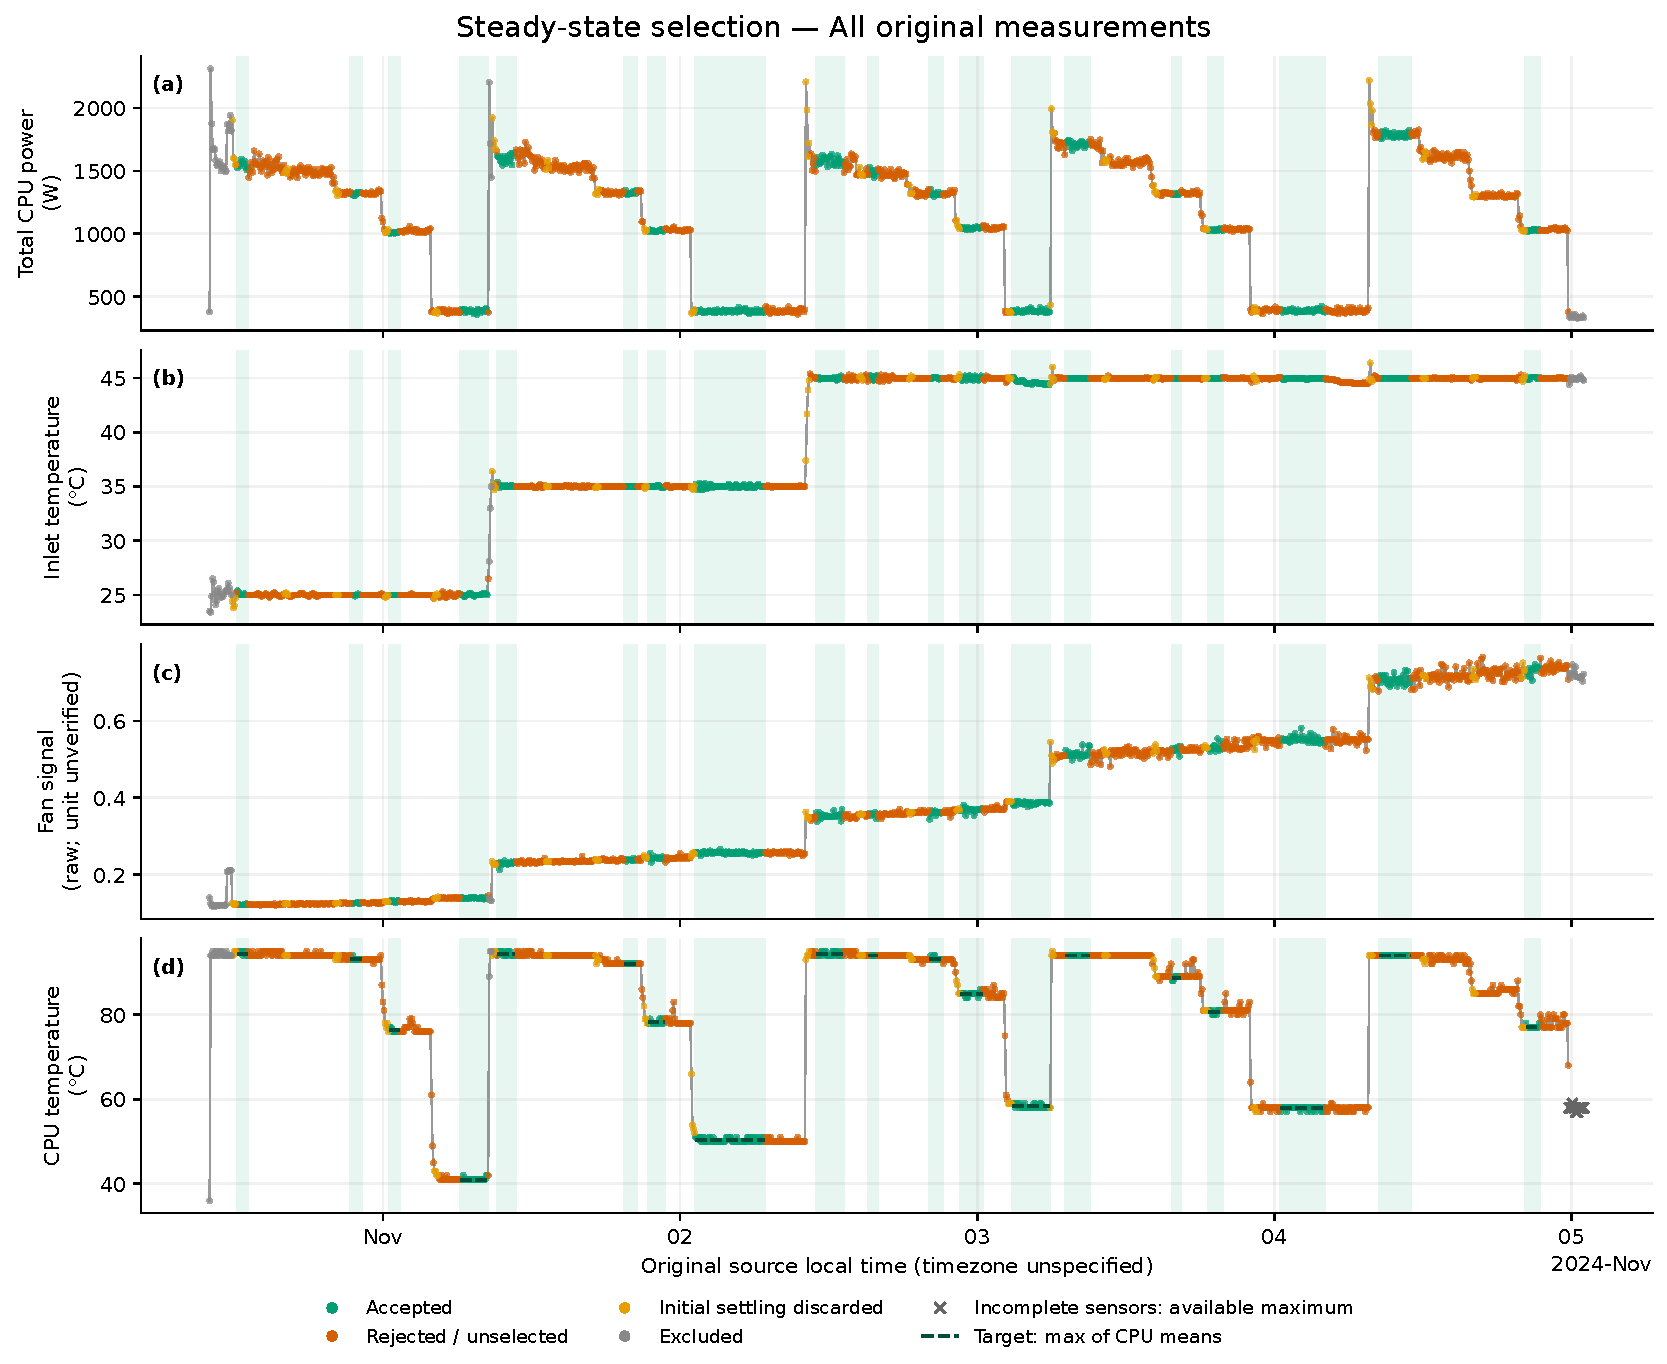
\includegraphics[width=\linewidth,height=50mm,keepaspectratio]
        {../../results/preprocessing/figures/selection_overview.pdf}
      \par\smallskip
      {\small\color{selectiongreen}\textbf{One green band = one processed observation.}}
      \par\smallskip
      {\footnotesize \textbf{60-minute dwell: 14 observations} (backup).}

    \column{0.41\textwidth}
      \begin{beamercolorbox}[sep=2mm,wd=\linewidth]{data panel}
        {\color{rwth-blue-100}\fontsize{22}{25}\selectfont\bfseries 19}\par
        \textbf{operating observations}\par
      \end{beamercolorbox}
      \medskip
      \dataheading{Each observation contains:}
      \footnotesize
      \[
        \Bigl(
          \underbrace{\bar P_{\mathrm{CPU}},\,\bar T_{\mathrm{inlet}},\,\bar F}_{\text{three inputs}},\;
          \underbrace{\max_{j=1,\ldots,18}\bar T_j}_{\text{temperature target}}
        \Bigr)
      \]
      Interval averages; $j=1,\ldots,18$ indexes CPUs.
      \par\smallskip
      \begin{beamercolorbox}[sep=1.5mm,wd=\linewidth]{data warning}
        \dataheading{Our starting choice: degrees 1 and 2}
        \footnotesize
        \begin{itemize}
          \item Full bases: \textbf{4 / 10 coefficients}; cubic: 20 ($>19$).
          \item Quadratic design: $\kappa_2\approx702$; coefficients may be unstable.
          \item Higher degrees need sparsity / regularization; validate either choice.
        \end{itemize}
      \end{beamercolorbox}
  \end{columns}
\end{frame}
